\renewcommand{\thesection}{S\arabic{section}}
\setcounter{section}{5}
\section{Sensitivity Analysis}
\label{sec:Appendix_S6}

The preceding analyses assume that the delay distribution \(g(\tau)\) is known. In practice, however, epidemiological delay distributions must be estimated from finite and often right-truncated data, introducing uncertainty in both the location and dispersion of the delay process. Because the delay kernel determines the frequency-dependent attenuation factor \(|\widehat G(f)|^2\), uncertainty in the assumed delay distribution changes the amount of upstream information that survives to the downstream observations and therefore shifts the quantitative boundary of statistical identifiability.

To quantify this effect, we evaluated the sensitivity of the minimum required frequency-domain contrast-to-noise ratio for statistical distinguishability. Under the separability criterion developed in the main text, the minimum upstream contrast required for distinguishability at frequency \(f\) is

\begin{equation}
Q_{\min}(f)
=
\frac{\tau_{M,\alpha}}
{p^2|\widehat G(f)|^2},
\end{equation}

where \(\tau_{M,\alpha}\) denotes the observation-model-specific non-identifiability threshold corresponding to the target testing-error level \(\alpha\). Larger values of \(Q_{\min}\) therefore indicate that increasingly larger upstream spectral contrast, relative to the effective downstream noise level, is required for statistical distinguishability.

Figures~\ref{fig:delay-sensitivity}A--C show the resulting \(\log_{10}(Q_{\min})\) across a family of lognormal delay distributions parameterized by their median delay and dispersion factor. For all perturbation periods, the required contrast-to-noise ratio increases as either the median delay or the dispersion increases, reflecting progressively stronger attenuation of upstream temporal variation. The effect is strongest for short-period perturbations. For 3-day variation, moderate changes in the delay distribution shift the required contrast-to-noise ratio by several orders of magnitude, whereas 14-day perturbations remain comparatively insensitive across a much broader region of parameter space.

The empirical delay estimates shown in Figures~\ref{fig:delay-sensitivity}A--C occupy markedly different regions of this identifiability landscape. Delays associated with long reporting processes, such as dengue and Ebola surveillance, lie in regions requiring substantially larger upstream contrast for short-timescale distinguishability, whereas incubation-period delays for respiratory infections occupy regions with considerably lower requirements. These differences arise directly from the frequency responses of the corresponding delay kernels.

We next examined the local sensitivity of the identifiability boundary around each empirical delay estimate. For every disease, we perturbed either the median delay or the dispersion parameter while holding the remaining parameter fixed and recomputed the corresponding minimum required contrast-to-noise ratio. Figures~\ref{fig:delay-sensitivity}D--F summarize the resulting change,

\begin{equation}
\Delta\log_{10}Q_{\min}
=
\log_{10}
\left(
\frac{Q_{\min}}
{Q_{\min,0}}
\right),
\end{equation}

where \(Q_{\min,0}\) denotes the value obtained under the original delay estimate.

Misspecification of the median delay produces substantial changes in the identifiability boundary for short-period perturbations. For several representative delay distributions, a moderate shift in the assumed median delay changes the required contrast-to-noise ratio by more than an order of magnitude for 3-day perturbations. The corresponding effect is considerably smaller for 7-day and 14-day variation, indicating that longer-timescale signals remain substantially more robust to uncertainty in delay location.

A similar pattern is observed for uncertainty in the dispersion parameter (Figures~\ref{fig:delay-sensitivity}G--I). Increasing dispersion consistently raises the required contrast-to-noise ratio because broader delay distributions more strongly suppress high-frequency upstream variation. Once again, this effect is concentrated near the temporal-resolution limit imposed by the observation process and becomes progressively weaker for longer-period perturbations.

Taken together, these results demonstrate that uncertainty in the delay distribution primarily influences the quantitative location of the identifiability boundary rather than the qualitative conclusions of the framework. Moderate uncertainty in delay estimation has relatively little effect on long-timescale epidemic variation but can substantially alter the amount of upstream contrast required to distinguish rapid fluctuations from observational noise. Consequently, inference concerning short-timescale epidemic dynamics should be interpreted together with uncertainty in the assumed delay distribution.

\begin{figure*}[!t]
    \centering
    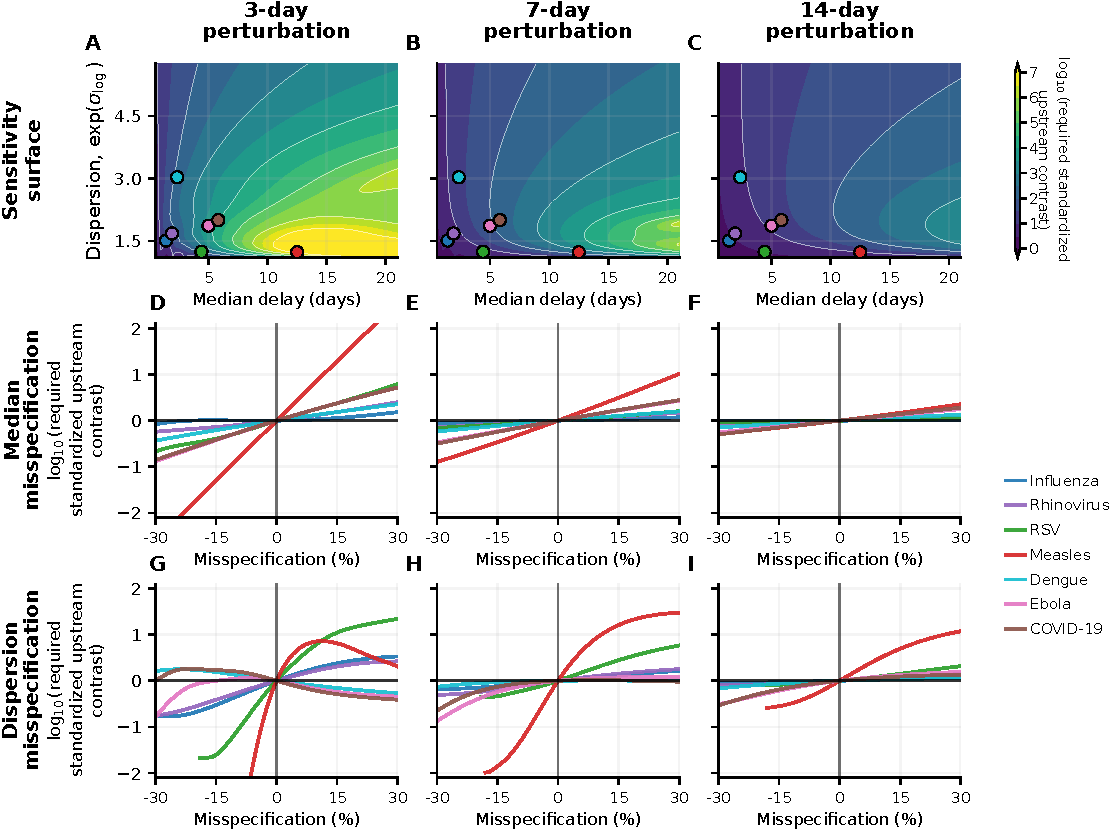
\includegraphics[width=\textwidth]
    {figs/sensitivity_analysis.pdf}
    \caption{
    \textbf{Sensitivity of spectral identifiability to uncertainty in the delay distribution.}
    (A--C) Global sensitivity landscapes showing the minimum required frequency-domain contrast-to-noise ratio for statistical distinguishability across lognormal delay distributions parameterized by median delay and dispersion factor. Results are shown for upstream perturbations with characteristic periods of 3, 7, and 14 days. Colored points indicate representative empirical delay estimates.
    (D--F) Sensitivity to uncertainty in the median delay while holding the dispersion factor fixed.
    (G--I) Sensitivity to uncertainty in the dispersion factor while holding the median delay fixed. Rapid perturbations are substantially more sensitive to delay uncertainty than longer-timescale perturbations, although the magnitude of this sensitivity depends on the underlying delay distribution.
    }
    \label{fig:delay-sensitivity}
\end{figure*}